% Text for the introduction section
\lettrine{F}{or} more than half a century, humans have envisioned a future where every person would have a personal air vehicle for transportation, often envisioned as a flying car.
Henry Ford stated in 1940: ``Mark my word: a combination airplane and motorcar is coming. You may smile, but it will come.''\cite{schilling2001looking}
While this future has yet to come to pass, recent developments in aviation and technology have made this reality closer than ever. 
The vision now is for an urban air taxi service (also commonly referred to as urban air mobility or UAM) capable of shuttling passengers around metropolitan areas thereby escaping the road congestion below.\cite{moore2003personal}
This vision has sparked the development of a number of UAM concept vehicles within industry and at NASA.
These vehicles are typically vertical take-off and landing (VTOL) designs which which are capable of carrying 1 to 30 passengers in an intra-urban environment on flights of less than 50 nautical miles. 

Within NASA, three UAM concept vehicles have been developed by the Revolutionary Vertical Lift Program to focus and guide research activities.\cite{johnson2018concept}
These vehicles, shown in Figure \ref{f:UAM}, differ significantly in their design, size, payload, range, propulsion system and operation.
The concept on the left is a quadrotor vehicle designed to carry a single passenger over a short 50 nm range.  
Because of this short range and small size, it is anticipated that the propulsion system for this vehicle would be all-electric.
The vehicle on the right is the next largest with the ability to carry six passengers over four 50 nm flight segments before needing refueling.
% The mission profile for this vehicle (and the segments for the other vehicles) is shown in Figure \ref{f:profile}. 
This concepts is envisioned to have a hybrid propulsion system with some power produced by energy stored in batteries with the rest coming from turboshaft engines.
Lastly, the largest concept in the center is a tiltwing design capable of carrying 15 passengers on eight 50 nm flight segments.
The propulsion system for this concept is expected to be a turboelectric design where a single turboshaft engine generates electricity which is transmitted four electric motor driven rotors/propellers.
% The propulsion system for this turboelectric tiltwing concept is shown in Figure \ref{f:turboelectric}.
It is this last concept, the turboelectric tiltwing, which will serve as the demonstration example in this paper.

\begin{figure}
\begin{center}
 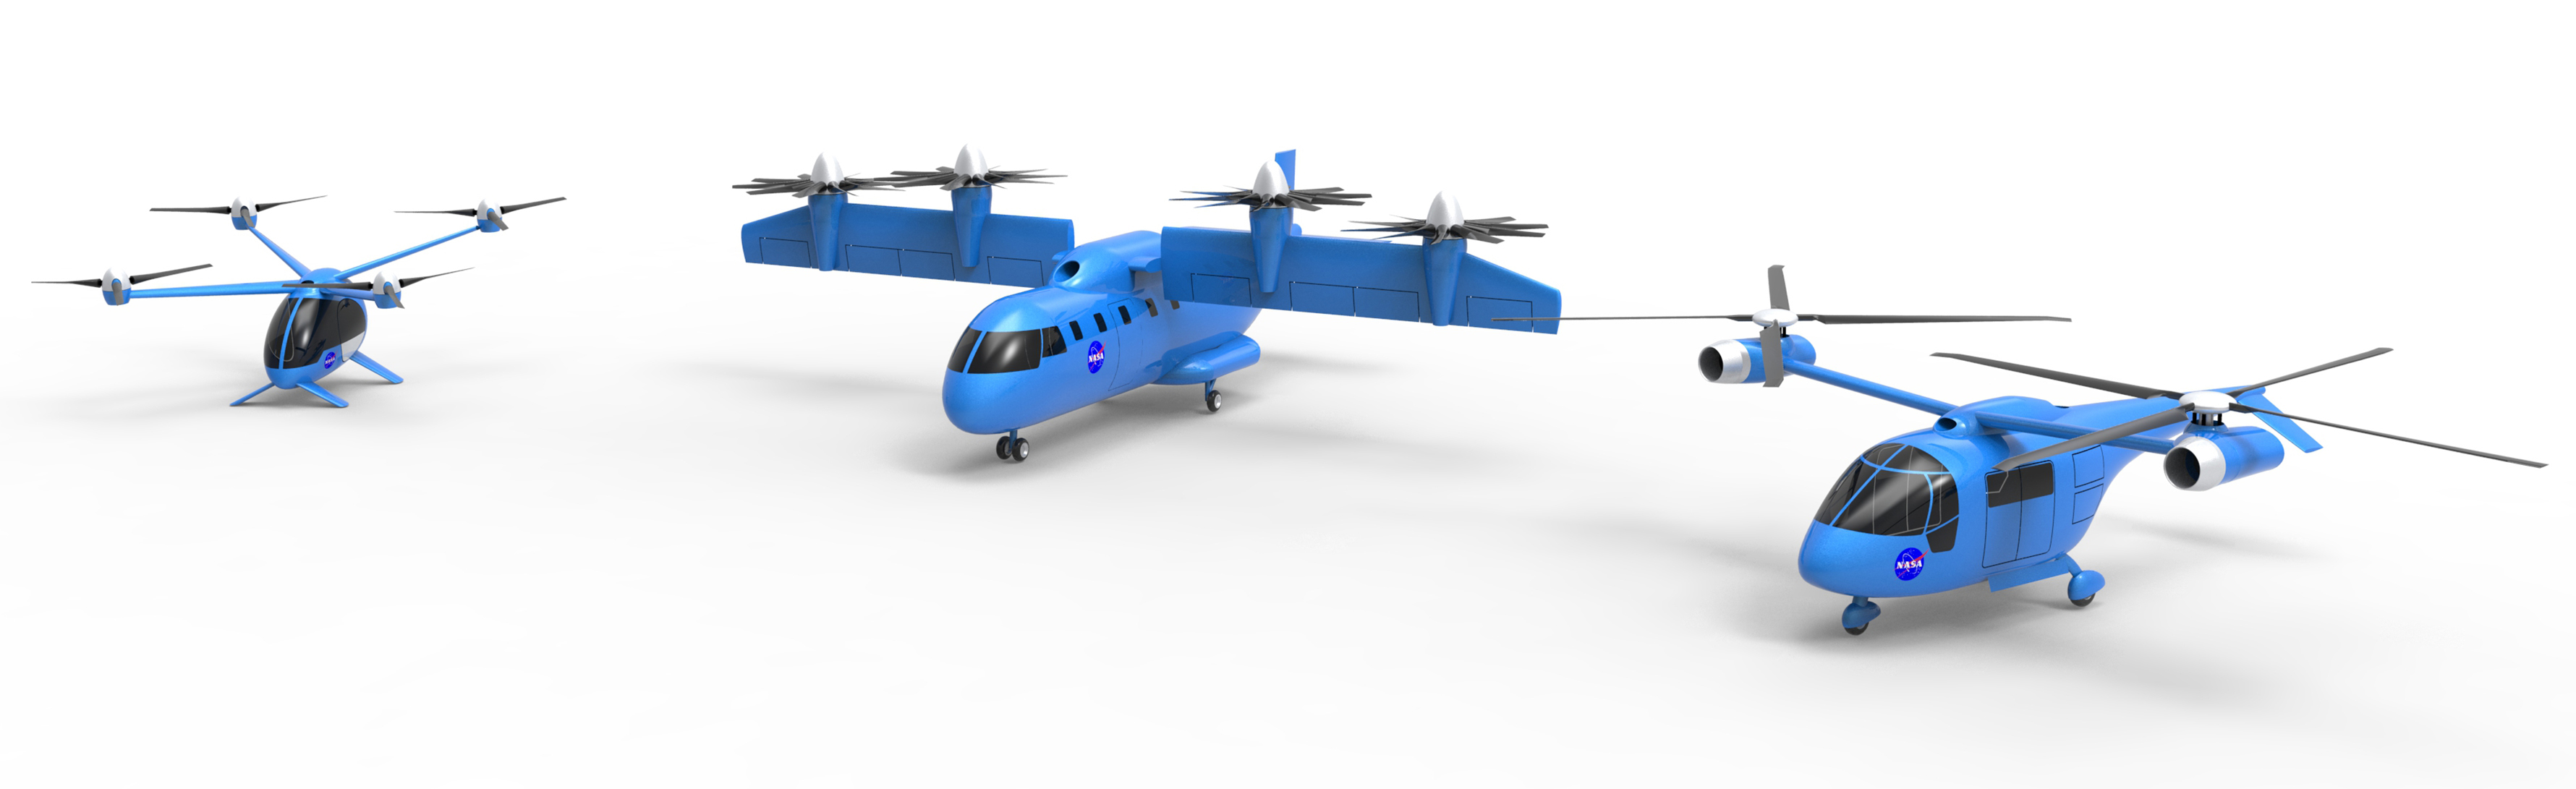
\includegraphics[width=1.0\textwidth]{../Images/UAM_GROUP1.jpg}
 \caption{NASA Urban Air Mobility Concept Vehicles.}
 \label{f:UAM}
\end{center}
\end{figure}

% \begin{figure}
% \begin{center}
%  \includegraphics[width=0.6\textwidth]{../Images/Mission_profile.pdf}
%  \caption{Mission Profiles for UAM Concept Vehicles.\cite{johnson2018concept}}
%  \label{f:profile}
% \end{center}
% \end{figure}


% The purpose behind NASA developing these designs is to focus and guide NASA research on the technologies needed to make UAM become a reality.\cite{johnson2018concept}
The initial studies to develop these UAM concept vehicle designs applied a set of existing rotorcraft design and analysis tools in a traditional design process.
Overall, the the objectives of these studies were to sufficiently refine the design such that crucial technologies and research needs could be identified. 
Therefore, from the concept designs generated several areas of further research which are required to evolve and mature the designs were identified.
These areas included improving the modeling and assumptions for the propulsion system, vehicle weights, aerodynamics and acoustics.\cite{johnson2018concept}
Furthermore, it was identified that the traditional design process needs to be modified to perform an integrated multidisciplinary environment to optimize these concepts to further improve the overall design

Given these needs, this work presents the development of a multidisciplinary analysis environment which can be used to support the conceptual design of UAM vehicles.
This multidisciplinary analysis and design environment provides improved modeling capabilities for disciplines including modeling the aircraft trajectory, propulsion system, electrical system, structures and aerodynamics. %potentially add TMS and the acoustics if they end up in the models for this paper
These disciplinary modeling tools are developed with the ability to compute analytic derivatives to support the close coupling of the tools within a larger multidisciplinary environment.
The analytic computation of derivatives is a key feature of this tool suite as it provides enhanced capabilities for gradient-based optimization of the multidisciplinary model. 

This paper is organized as follows:
Section \ref{sec:trad_process} first presents the traditional design process and tools used in the initial design of the UAM concept vehicles.
Following this background, the development of the new multidisciplinary design, analysis and optimization (MDAO) environment and its supporting tools is summarized in Section \ref{sec:mdao_process}.
The features of the multidisciplinary analysis environment are then demonstrated by applying it to the optimization of the turboelectric tiltwing UAM vehicle described above in Sections \ref{sec:opt_prob} and \ref{sec:opt_results}.
Following this optimization demonstration, conclusions and future work are discussed in Section \ref{sec:conc}. 

